\begin{figure}
    \centering
  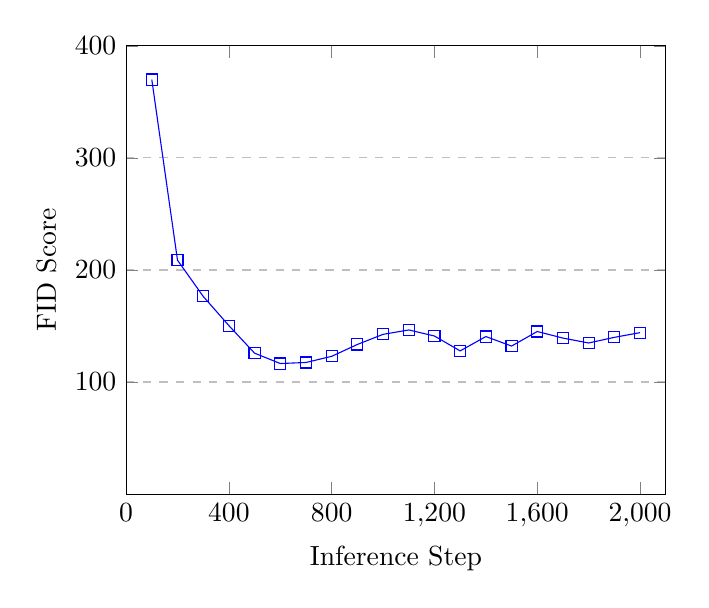
\begin{tikzpicture}
  \begin{axis}[
      xlabel={Inference Step},
      ylabel={FID Score},
      xmin=0, xmax=2100,
      ymin=0, ymax=400,
      xtick={0,400,800,1200,1600,2000},
      ytick={100,200,300,400},
      ymajorgrids=true,
      grid style=dashed,
  ]
  
  \addplot[
      color=blue,
      mark=square,
      ]
      coordinates {
        (100,369.88)(200,208.77)(300,176.46)(400,150.36)(500,125.77)(600,116.52)(700,117.46)(800,122.95)(900,133.55)(1000,142.56)(1100,146.5)(1200,141.07)(1300,127.79)(1400,140.6)(1500,132.09)(1600,145.1)(1700,139.23)(1800,134.86)(1900,139.89)(2000,144.07)
      };
      
  \end{axis}
  \end{tikzpicture}
  % 对于Oxford Flower数据集,随着噪音添加次数的增加,由扩散模型生成的图像的FID得分发生的变化。
    \caption{For the Oxford Flower dataset, as the number of noise additions increased, there was a change in the FID score of the images generated by the diffusion model.}
    \label{fig:flower_fid}
  \end{figure}